\documentclass[twocolumn]{jarticle}
\usepackage[dvipdfmx]{graphicx}
\usepackage{appi2013_2}

%%packages related to equations and math letters
\usepackage{amsmath,amssymb,amsfonts}
\usepackage{amsthm} %定理環境.
%\usepackage{theorem} %定理環境.amsthmを使う場合はコメントアウト.
\usepackage{siunitx} %単位,数値に必要.
\usepackage{latexsym}
\usepackage{empheq} %連立方程式に用いる
%\usepackage{array} %連立方程式に用いる.empheq環境でよい.
%%

%packages related to fonts
\usepackage{bm}
\usepackage{bbm}
\usepackage{otf}
\usepackage[dvipdfmx]{color}
\usepackage[version=3]{mhchem} %化学式を出力するときに用いる.
%\usepackage{newtxtext,newtxmath} %Times フォント関係のパッケージ.
\usepackage{times} % TimesとHelveticaを使う。数式はComputer Modern
%%

%%packages related to structure of the text
\usepackage{ascmac} %make frames
\usepackage{enumerate} %make lists
%\usepackage{enumitem} %customize package of enumerate
%%
%%packages related to quote
%\usepackage{cite}
\usepackage{url}
\usepackage[superscript]{cite}  %参考文献番号を上付にしないなら要らない
\renewcommand\citeform[1]{[#1]} %cite.styを使わないときにはこれもコメントにすること
%%

%%packages related to algorithm and source code
\usepackage{algorithm}
\usepackage{algorithmic}
%\usepackage{listings}
%%

%%packages related to figures and tables
\usepackage{wrapfig}
\usepackage{subcaption}
\usepackage{here}
%\usepackage{multirow}
%\usepackage{slashbox}
%\usepackage{longtable}
%\usepackage{float} %here環境と同じ.使う必要はない.
%%
%%package related to comment
\usepackage{comment} %\begin{comment} ~ \end{comment}でコメントアウトできる.
%%
%%package related to pdf
%\usepackage{pdfpages}

\usepackage{mathtools}
\usepackage[labelformat=parens, justification=raggedright]{subcaption}
% \newcommand{\rfig}[1]{Fig.~\ref{#1}}
% \newcommand{\req}[1]{式\eqref{#1}}
%%command to erase trivial cautions  
\DeclareFontShape{JY1}{hmc}{b}{n}{<->ssub*hmc/bx/n}{} % Font shape `JY1/hmc/b/n' undefined (Font) using `JY1/hmc/bx/n' instead.のエラーメッセージを消すコマンド.
\DeclareFontShape{JT1}{hmc}{b}{n}{<->ssub*hmc/m/n}{} %LaTeX Font: Font shape `JT1/hmc/b/n' undefined (Font)	using `JT1/hmc/m/n' instead.のエラーメッセージを消すコマンド.
%%


\jtitle{\fontsize{13pt}{0pt}相互通信可能な分子通信系シミュレーションによる濃度依存性の検証}
\etitle{Two-step reinforcement learning for model-free redesign of nonlinear optimal regulator}
\lab{堀}
\no{82411805}
\name{川口竜輝}
\begin{document}
\maketitle

\section{研究背景・目的}
自然界において,細胞はシグナル分子と呼ばれる伝達物質を別の細胞に送ることで
情報の伝達を行っている.このような細胞間の情報伝達を相互に行う系は分子通信系と呼ばれ,
系は細胞内での化学反応と細胞間のシグナル分子の伝達によって構成されている.
分子通信系では,系内部の細胞の濃度が系全体の状態に影響を与えることが知られているが,
その量的な関係を調べた研究は少ない.


\section{相互通信可能な分子通信系}
% 状態$\bm{x}_{k} \in \mathbb{R}^{n}$,入力$\bm{u}_{k} \in \mathbb{R}^{m}$に関するコスト関数
% \begin{align}
%     \sum^{\infty}_{k=0} \gamma^{k} (\bm{x}_{k}^\top Q \bm{x}_{k} + \bm{u}_{k}^\top R \bm{u}_{k})
%     \label{eq:cost_equation}
% \end{align}
% を最小にするような制御器を設計する問題を考える.ただし,$Q \in \mathbb{R}^{n \times n}, R \in \mathbb{R}^{m \times m}$はそれぞれ半正定値,正定値行列であり,$\gamma \in (0, 1)$は
% %割引率と呼ばれる
% 定数である.
% この問題に対し,\rfig{fig:proposed_method}で表される制御器の設計を2つのステップに分けて行う.

% Step~1ではまず,既知の安定なフィードバックゲイン$K^{\mathrm{init}}$を用い,探索項を印加しながらシステムを動かすことで入力と状態の時系列データを取得する.
% その後,ベルマン方程式から導出される関係式
% \begin{align}
% F ^j [\textrm{vec}(G^{j+1}_1)^\top ,\textrm{vec}(G^{j+1}_2)^\top ,\textrm{vec}(G^{j+1}_3)^\top]^\top=\bm{h}^j
% \label{update_equation}
% \end{align}
% によって$G^{j+1}_i,~i=1,2,3$
% を更新し,
% $K^{j+1}=-(R+G_3^{j+1})^{-1}G_2^{j+1}$
% % \begin{align}
% %     K^{j+1}=-(R+G_3^{j+1})^{-1}G_2^{j+1}
% % \end{align}
% に代入することで
% %フィードバックゲイン
% $K^j$の更新を行う.
% ただし,$\bm{h}^{j}$は各時刻における
% 二次コストに関するベクトル,
% $F^{j}$は入力と状態に関する行列,
% $G^{j+1}_i$は
% コスト関数に関する行列であり,
% $F^j,~ \bm{h}^j$は取得した時系列データと$K^j$から計算される.
% $||K^j-K^{j-1}||$が閾値以下になったら更新を終了し,このときの$K^j$を$K^{\rm{AC}}$とする.更新される$K^{j}$は,準最適線形LQR制御則に収束する.

% Step~2では,Step~1で設計された線形制御器と並列に繋げた非線形制御則$\bm{\mu}$を強化学習の一種であるActor-Critic法\cite{Sutton_RL}によって設計する.
% 線形制御則$K^{\rm{AC}}$が存在することで,学習中にシステムが不安定になることを防ぎ,損耗を防ぐことができる.
% この二段階の設計手法による制御則は,線形制御則だけでは実現できない性能を達成する.

\begin{figure}[tb]
    \centering
    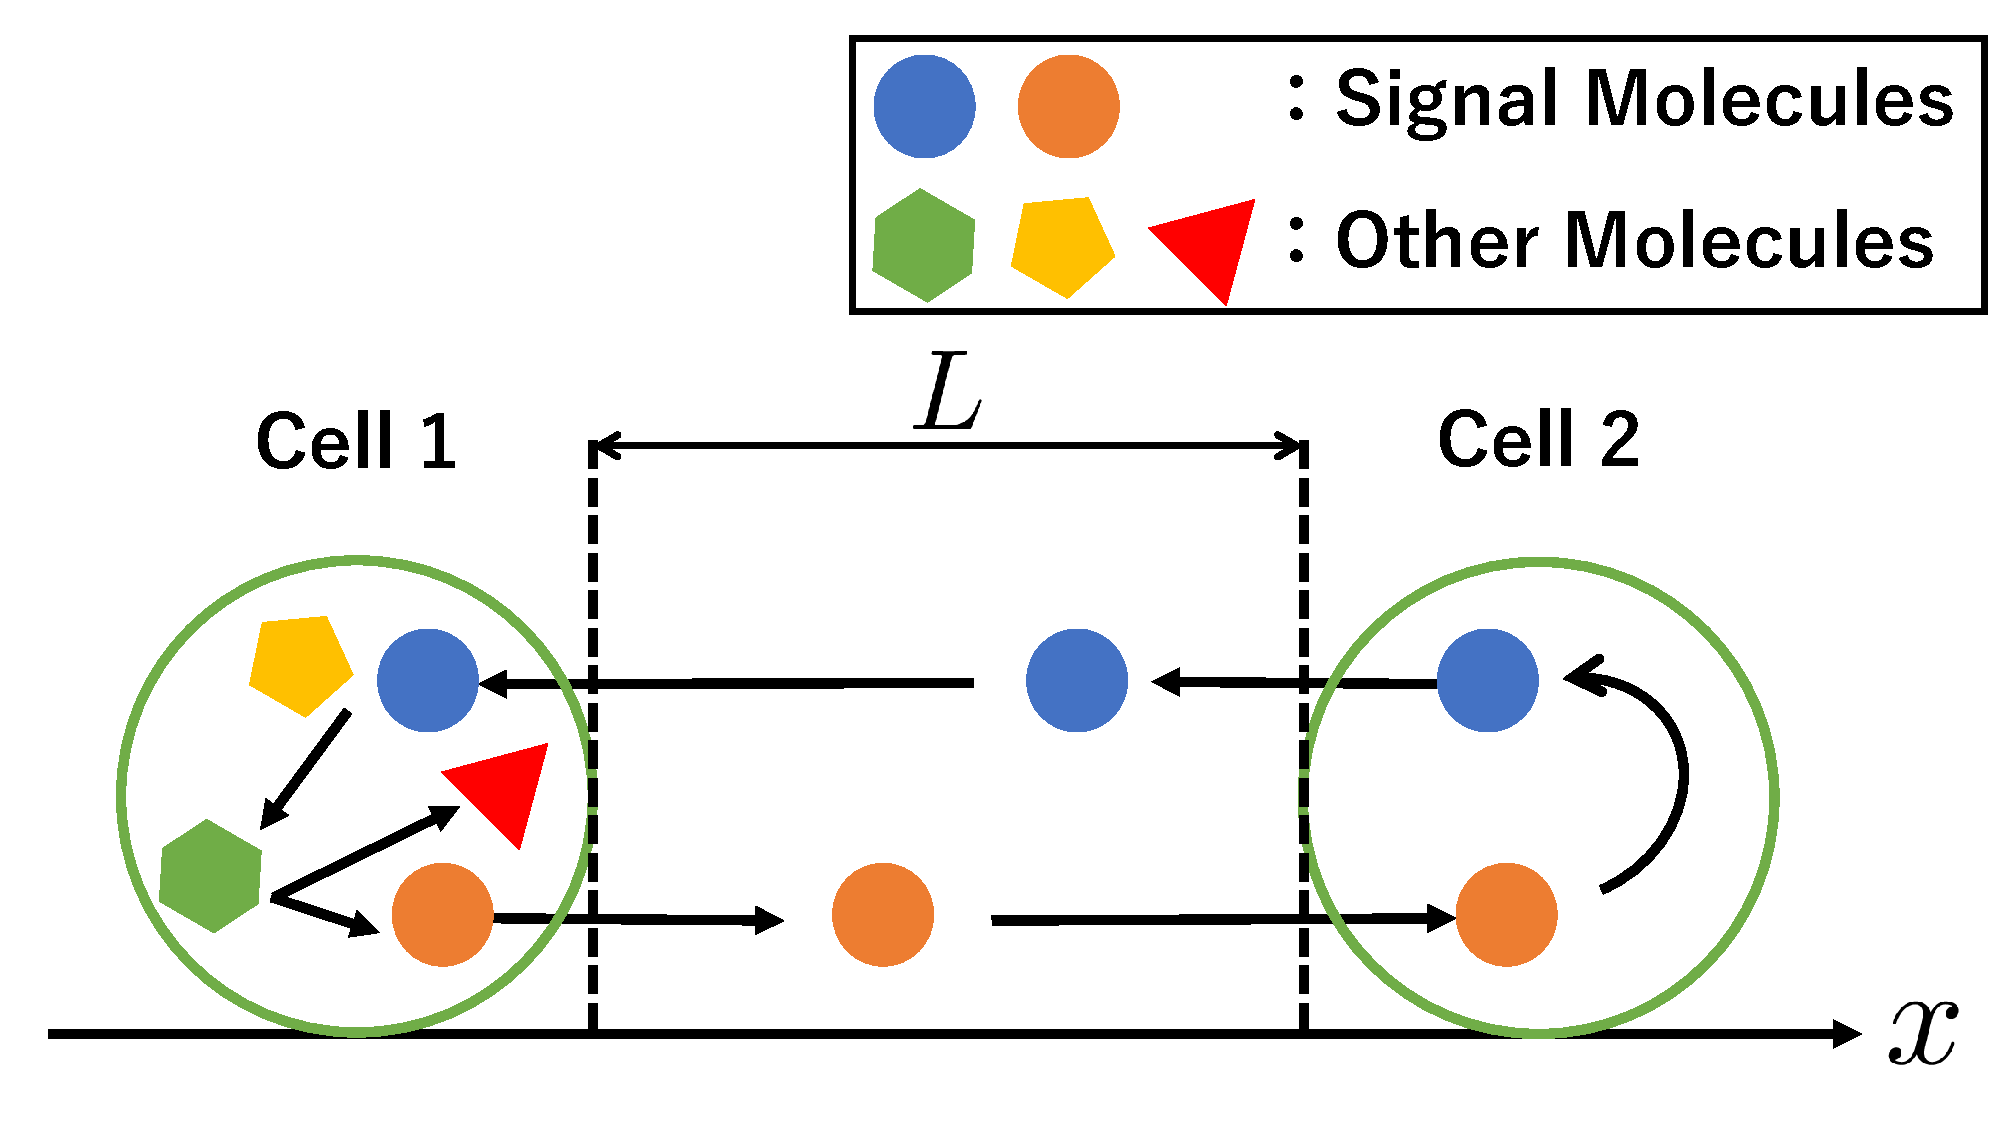
\includegraphics[width=\columnwidth] {figures/Images.pdf}
    \caption{Image of 1 dimension Molecular Communication System}
    \label{fig:image}
\end{figure}


\section{数値例による検証}
Fig. \ref{fig:image}にあるように,細胞が2つ存在する1次元の分子通信系を考える.ただし,系の拡散係数$\mu=$$3.0\times10^{-4}$,細胞間距離を$L$とする.
ここで細胞1内部には分子$\mathrm{A}$,$\mathrm{B}$,$\mathrm{X}$が存在し,次の細胞内部の反応によってシグナル分子$\mathrm{Y}$を放出する.
\begin{equation}
    \emptyset \xrightarrow{k_1} \mathrm{A},\mathrm{X}+\mathrm{A} \xrightarrow{k_2} \mathrm{B}, \mathrm{B} \xrightarrow{k_3} \emptyset, \mathrm{B}+\mathrm{B}\xrightarrow{k_4} \mathrm{B:B} +\mathrm{Y}
\end{equation}
細胞2内部には分子$\mathrm{Y}$が存在し,次の反応によってシグナル分子$\mathrm{X}$を放出する.
\begin{equation}
    \mathrm{Y} \xrightarrow{k_5} \mathrm{X}
\end{equation}
この時,時刻$t=0$において細胞$1$から分子$\mathrm{Y}$が$10^2$個放出されたとき,細胞$1$における分子$B$の時間発展を$1000$回シミュレーションし,
その平均を$L=\SI{0.1}{\um},$ $\SI{0.2}{\um},$ $\SI{0.3}{\um},$ $\SI{0.4}{\um},$ $\SI{0.5}{\um}$に対して計算した.
ただし,$k_1 = \SI{5.0}{\per\mm}$,$k_2 = \log(2)/20\ \si{\per\mm}$,$k_3=k_4=k_5=\SI{0.02}{\per\mm}$とした.
この時,各$L$に対する分子Bの時間発展をFig. \ref{fig:simulation}に示す.
Fig. \ref{fig:simulation}より,細胞間距離が短いほど分子Bの過渡応答が急峻であり,距離依存性を持つことが確認できる.

\begin{figure}[tb]
    \centering
    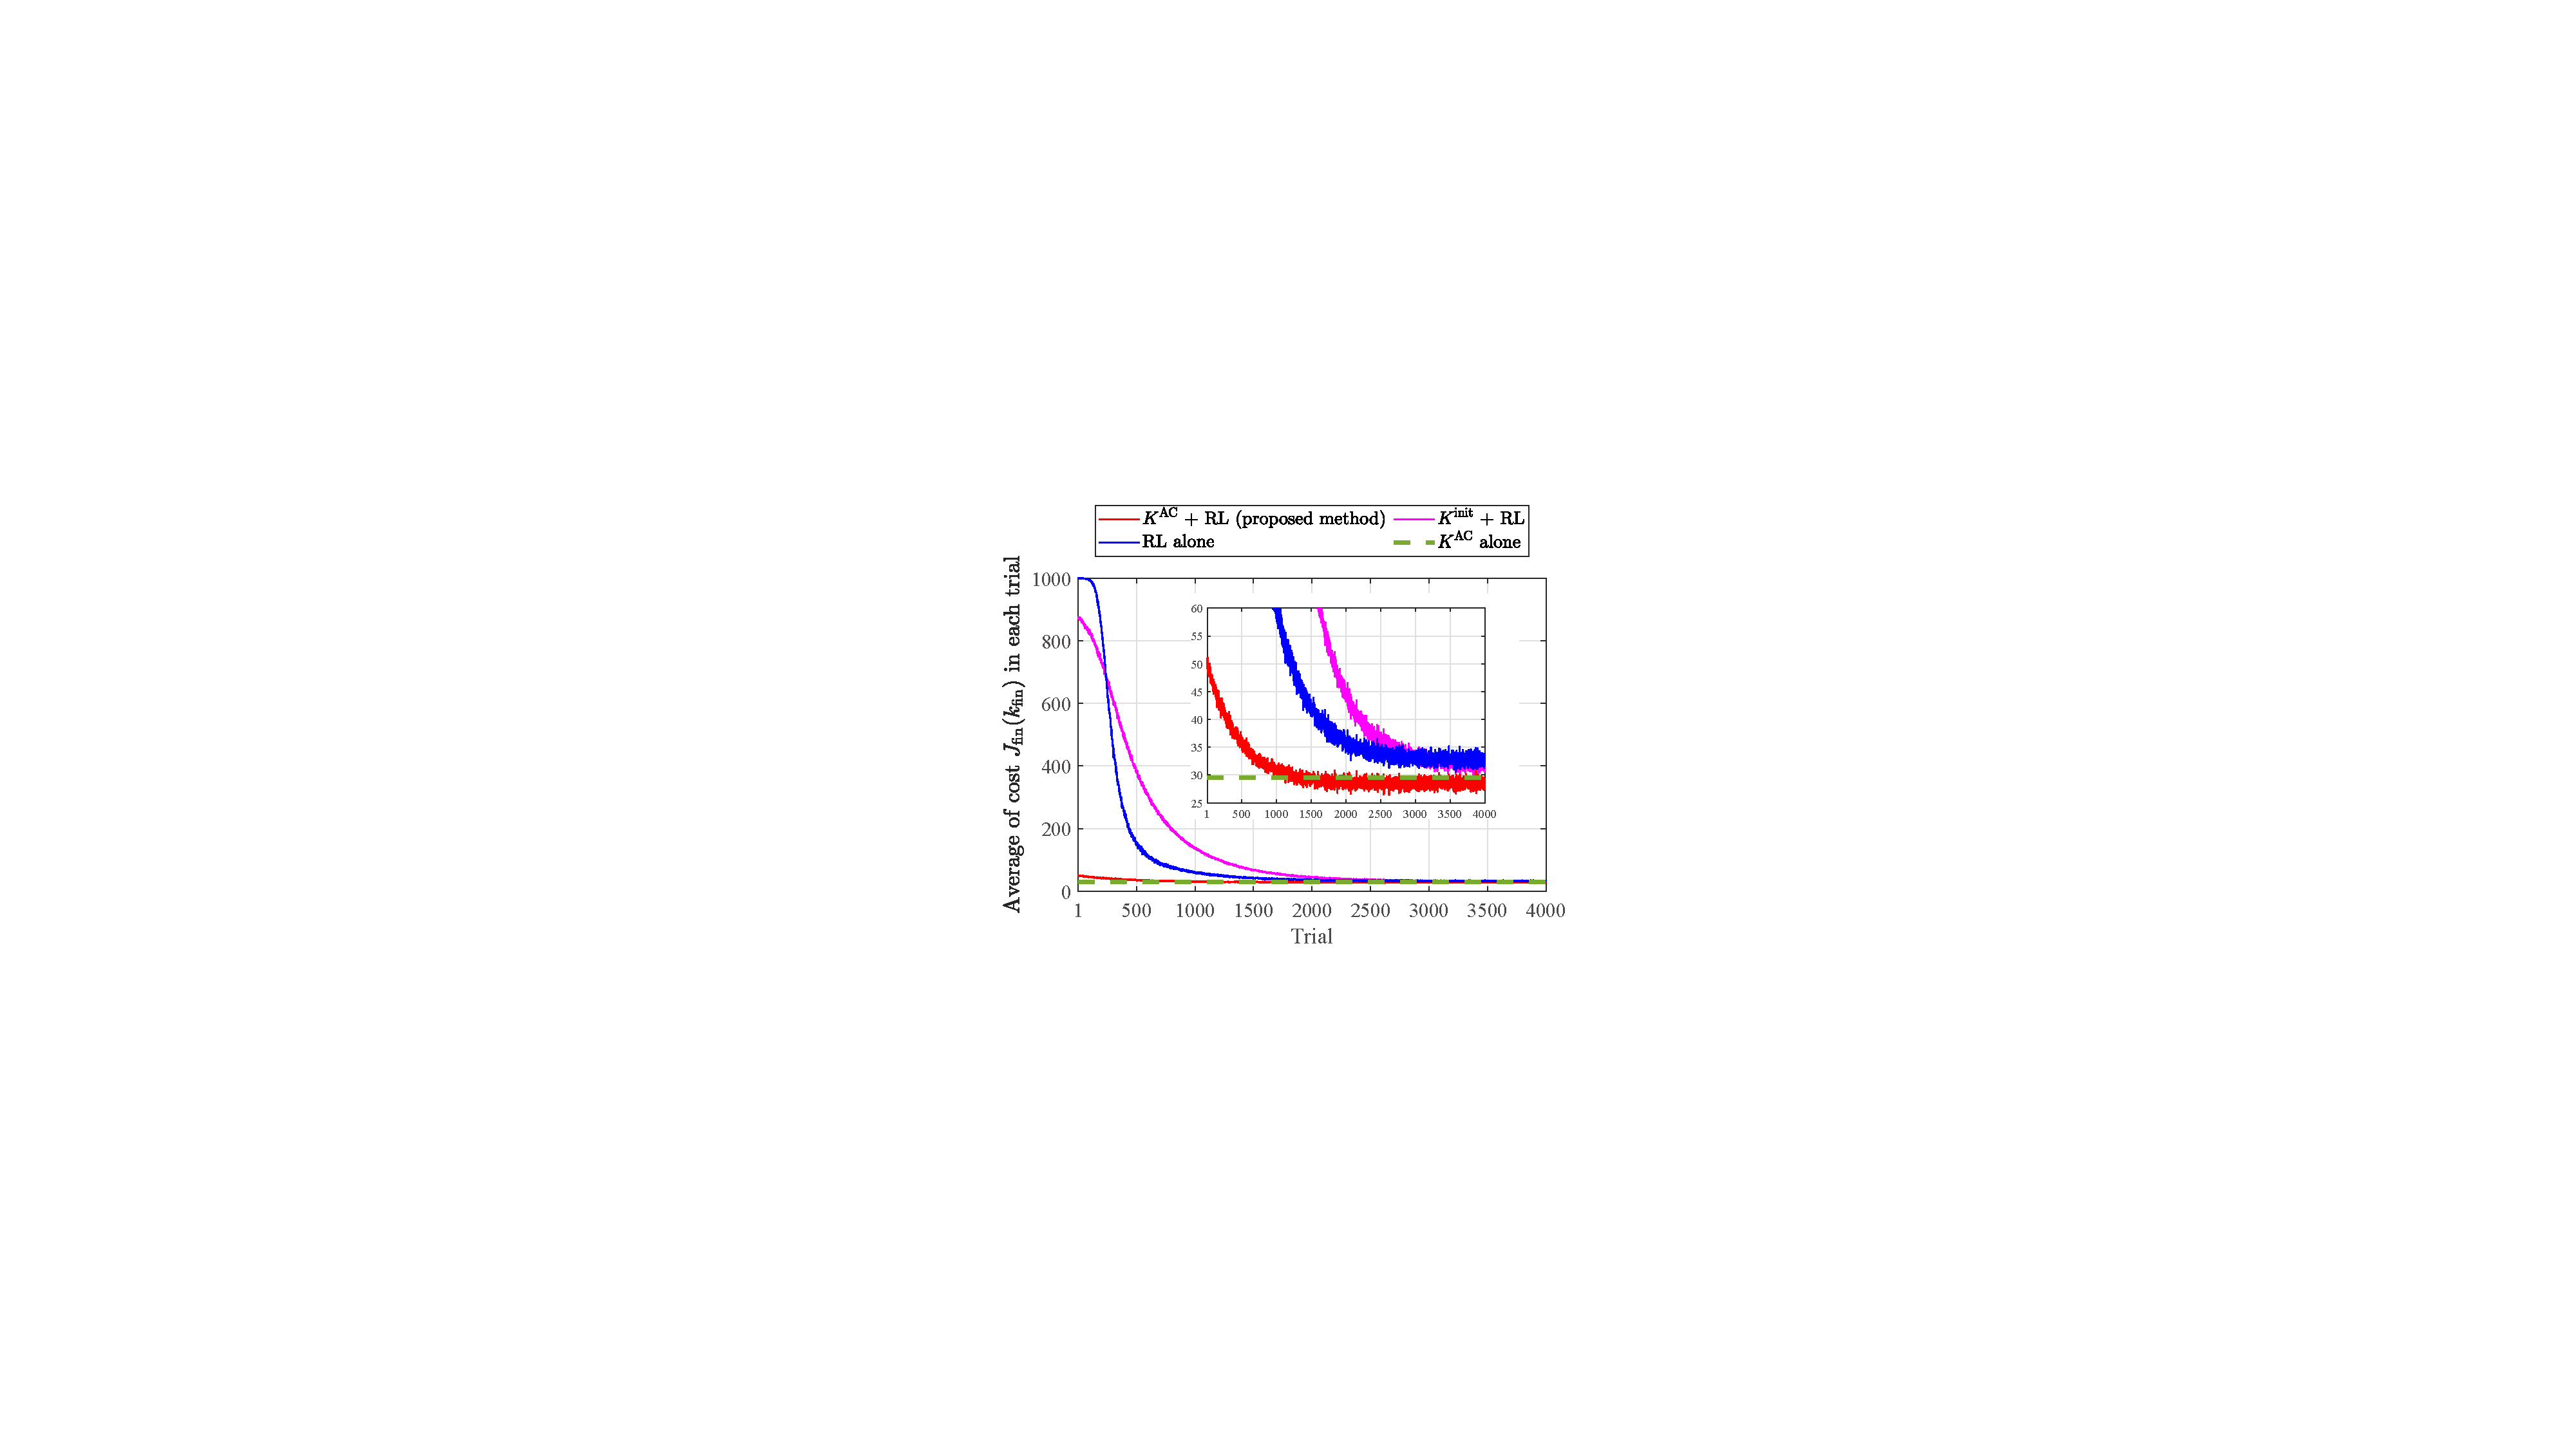
\includegraphics[width=\columnwidth]{figures/step2_cost_fig.pdf}
    \caption{Comparison of the time evolution of the average number of B among each $L$}
    \label{fig:simulation}
\end{figure}


\section{結論と今後の展望}
本稿では,相互通信可能な分子通信系のシミュレーション法による密度依存性の検証に向けて,
相互通信可能な1次元の分子通信系の数値シミュレーションを行った.
具体的には,送信細胞と受信細胞が固定されたシミュレーション法に対して,
シグナル分子の到達確率分布が分子の放出時刻だけシフトすることを利用して
相互通信可能な分子通信系のシミュレーションを提案した.
今後の展望としては,現在のシミュレーション法を利用して2次元の相互通信する分子通信系に対して
複数の濃度におけるシミュレーションを行い,濃度依存性の検証を行う.



\begin{thebibliography} {99}
    \bibitem{Sutton_RL} R. S. Sutton {\it et al}., %Reinforcement learning: An introduction,
    2nd ed. { \it MIT Press}, 2018.
    \bibitem{Kiumarsi2018} B. Kiumarsi {\it et al}., 
    %“Opti-mal and autonomous control using reinforcement learning: A survey, ”
    {\it IEEE Transactions on Neural Networks and Learning Systems}, vol. 29, no. 6, pp. 2042–2062, 2018.
\end{thebibliography}

\end{document}
